\documentclass[24pt, a0paper, landscape]{tikzposter}
\usepackage[utf8]{inputenc}
\usepackage{graphicx}
\usepackage{subcaption}
\usepackage[labelsep=period]{caption}
\usepackage{multicol}

\setlength{\columnsep}{3cm}

\usepackage{url}
\usepackage{hyperref}
\hypersetup{
colorlinks=true,
linkcolor=blue,
filecolor=magenta,
urlcolor=cyan,
}

\title{Nirdizati -- Anticipate the future {\LARGE \textit{(by training better models!)}} }
\author{Stanislav Mõškovski\\{\small \textit{Supervised by Ilya Verenich, MSc}}}
\date{today}
\institute{Institute of Computer Science, University of Tartu}


\begin{document}
    \maketitle

    \begin{columns}
        \column{0.3}
        \block{}
        {
        \begin{tikzfigure}
            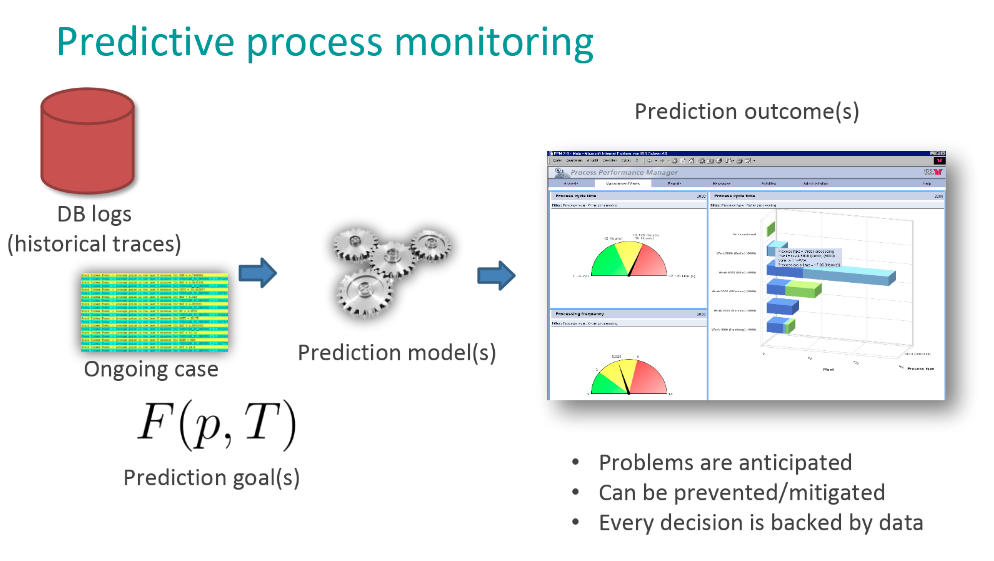
\includegraphics[scale=0.9]{figures/ppm.png}
        \end{tikzfigure}
        }

        \block{}
        {

        \begin{multicols}{2}
            {\huge\textbf{Problems}}
            \bigskip

            \begin{itemize}
                \item Processes take longer than necessary
                \item Deadline violations
                \item Process errors occur
                \item Inefficient resource management
            \end{itemize}
            \columnbreak

            {\huge\textbf{Solution}}
            \bigskip
            \begin{itemize}
                \item Predictive process monitoring
                \item Act before deviations happen
                \item Draw attention to potential problems
                \item Prioritize process instances
            \end{itemize}

        \end{multicols}

        }


        \block{Description}
        {
        \textbf{Nirdizati Training} allows business process analysts to easily \textbf{upload} their event log, \textbf{train}
        predictive models for various prediction targets by using state-of-the-art machine learning algorithms, \textbf{visualize and compare} the results
        and then \textbf{export} the model for further predictions on a live event stream.
        }

        \block{Advantages}
        {
        \begin{itemize}
            \item Accessible via any modern web browser that supports JavaScript
            \item Simple and sleek UI
            \item All computations are done of the server side
            \item Parallel training jobs
            \item Model accuracy visualization and comparison
            \item Great variety of machine learning techniques and algorithms
            \item Highly configurable training process for expert users
        \end{itemize}
        }

        \column{0.4}
        \block{User interface}
        {
        \begin{tikzfigure}[Training view of Nirdizati Training component]
            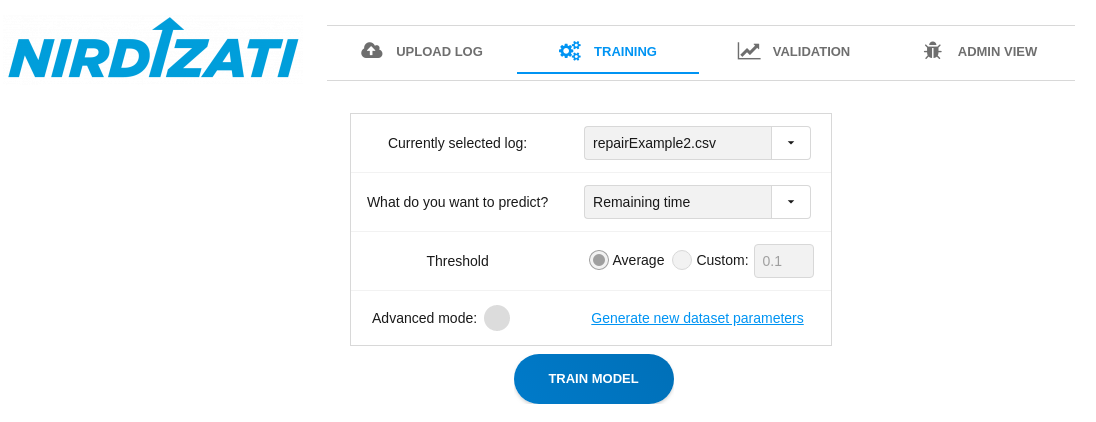
\includegraphics{figures/training.png}
        \end{tikzfigure}

        \begin{tikzfigure}[View of completed simulations, which allows sorting and grouping by various parameters.]
            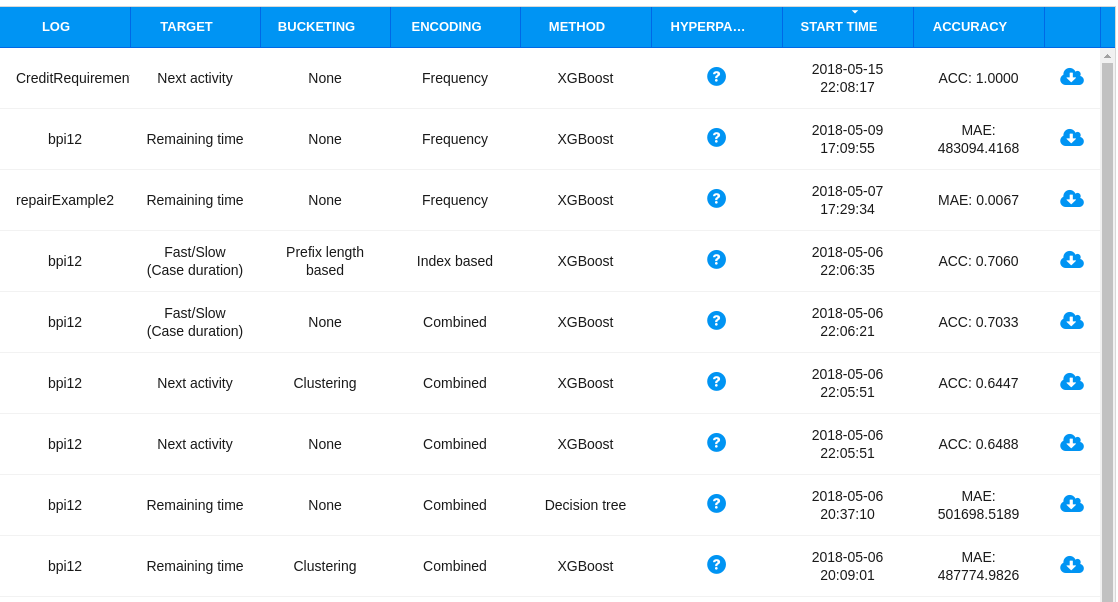
\includegraphics{figures/validation.png}
        \end{tikzfigure}

        \begin{tikzfigure}[Model evaluation view with model accuracy visualization]
            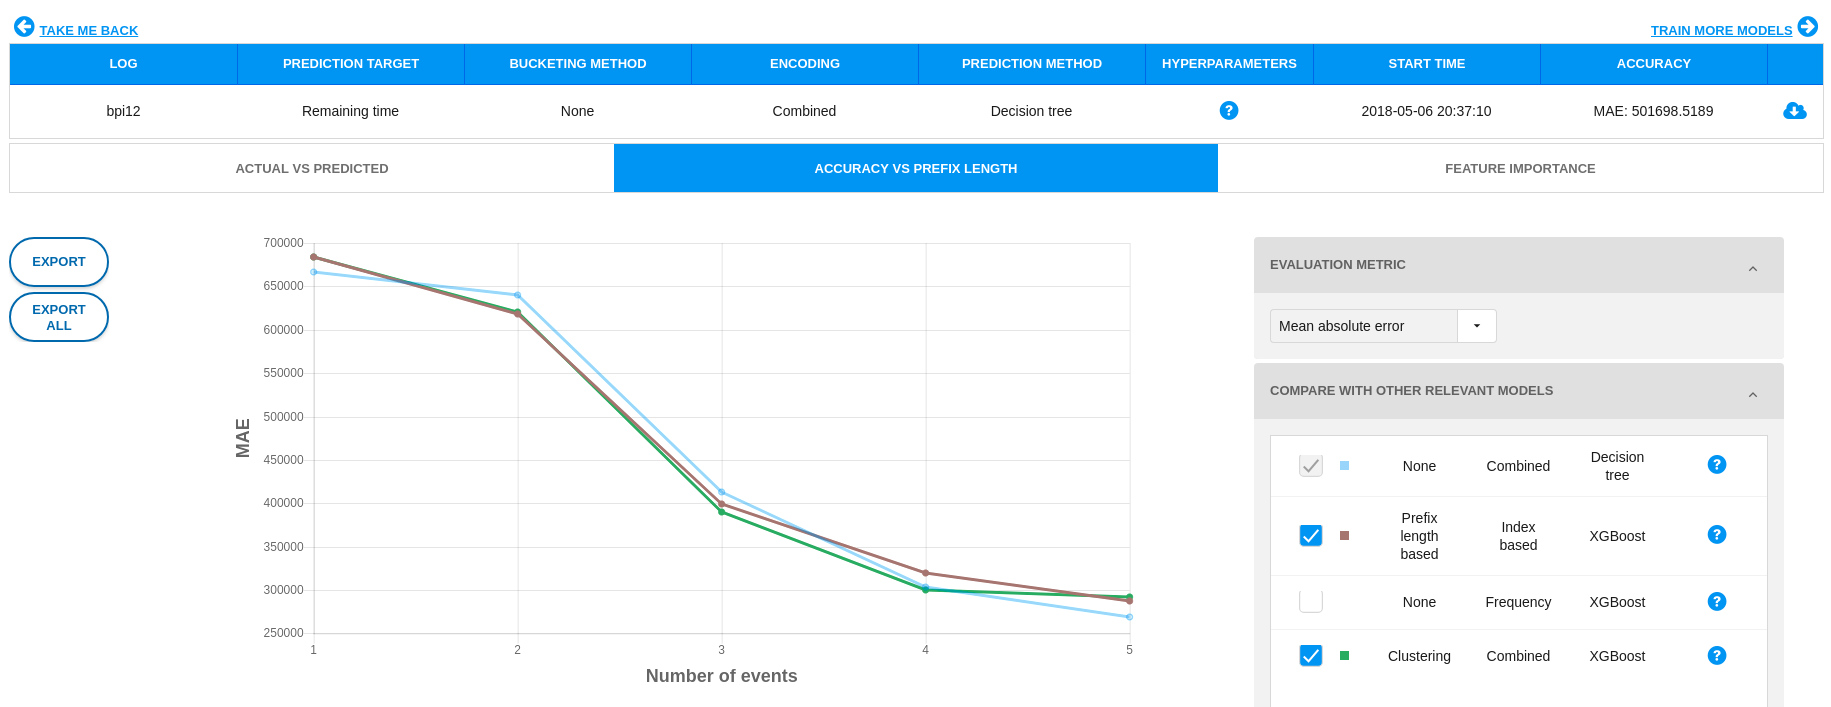
\includegraphics[scale=0.65]{figures/model_overview.png}
        \end{tikzfigure}
        }

        \column{0.3}
        \block{Technical solution}
        {
        \begin{tikzfigure}[Data flow of Nirdizati Training]
            \includegraphics[scale=0.7]{figures/data_flow.png}
        \end{tikzfigure}

        \begin{tikzfigure}[Architecture of Nirdizati Training]
            \includegraphics{figures/stack.png}
        \end{tikzfigure}
        }

        \block{Links}
        {
        	
       	\textbf{Live demo:} \href{http://training.nirdizati.org/}{\url{http://training.nirdizati.org/}}

        \bigbreak
        \textbf{Code:} \href{https://github.com/Zukkari/nirdizati-training-ui}{\url{https://github.com/Zukkari/nirdizati-training-ui}}
        
        \bigbreak
        \textbf{Landing:} \href{http://nirdizati.org/}{\url{http://nirdizati.org}}
        
        \bigbreak

        \textbf{Twitter:} \href{https://twitter.com/nirdizati}{\url{https://twitter.com/nirdizati}}
        }

        \block{}
        {

        \begin{multicols}{2}
            \begin{tikzfigure}
                
\includegraphics[scale=0.9]{figures/unilogo.jpg}
            \end{tikzfigure}

            \columnbreak

            \begin{tikzfigure}
                
\includegraphics[scale=0.5]{figures/qr.png}
            \end{tikzfigure}
        \end{multicols}

        }

    \end{columns}
\end{document}